\section{Instalación de Linux en SD para tarjetas Zybo}
\subsection{Instalación de Xillinux en tarjeta SD}
Para la instalación de Xiliniux, seguiremos los siguientes pasos:
\begin{itemize}
	\item Descargaremos una versión de Xillinux precompilada desde el siguiente \href{https://www.dropbox.com/s/9qgcoyjzoi764f0/2016.02.02.debian-cbaeef7e7f551052f5451957a5dbef43.zip?dl=0}{\textcolor{blue}{enlace}}.
	\item Descomprimimos el archivo descargado.
	\item Descargamos e instalamos el programa Win32 Disk Imager desde el siguiente \href{https://dw.uptodown.com/dwn/w76tVn7onjw1uZFTLSx7oG5vt1Y7gsfE_vPZCAa88I4YqL5Lp6S__CQhpJZGOLPYdjr73a4yGULPiRxv8Z2IsSRQjRPewPceg1Ol2gDzH3IkO3MHOCcuKQCNZwYI9Pvt/8_NYEhYYhGoJ_QXK-PQtvMDn5aHkqiWxwMofLuT2S5SxxDw2zu6f1OMCW0kqLnB0PGf-zrvou_F_nzjB4fn6Nuvp3WZcVrkFzGgNrhVLInDUMHPM0Jfxh76lJU_IATF7/9xrSlUN8npqZOVysN4LIc5iQnXIPmWNSWKNBLv7hcuQxXmyjX8qERxO48SnXIgr83mVVF-bcUsWJGGryhVqZ_LiBsoZmxxEyZE5JXoqVhCI=/}{\textcolor{blue}{enlace}}.
	\item Ejecutamos Win32 Disk Imager y seleccionamos la imagen descomprimida y la unidad de destino.
	\item Seleccionamos cread ``MD5 Hash'' para comprobar que la descarga no está corrupta. El resultado de dicho hash debe ser: ``cbaeef7e7f551052f5451957a5dbef43''.
	\item Pulsamos el botón ``\texttt{Escribir}'' para flashear la unidad seleccionada.
	\item Descargamos el archivo del kernel desde el siguiente \href{https://uc405c43ce82f6c3032b21ba76bf.dl.dropboxusercontent.com/cd/0/get/AehqJhpiTxZ90sAdGxOFqHxr04BAsug_4RaV6MPX5yBDOQBVaIpDw11X6LdVBi7DPsndN7IxeWYRcEmUAt4xnKoIeYJBRtYu4JtZ_M71as8xbw/file?_download_id=621489597300519201006251662619095482850364296264714456845096204891&_notify_domain=www.dropbox.com&dl=1}{\textcolor{blue}{enlace}}.
	\item Abrimos la carpeta contenedora de la tarjeta SD recién creada.
	\item Sobreescribimos los archivos de esa carpeta por los recién descargados del kernel\footnote{Si no se puede sobreescribir por falta de espacio, es preferible eliminarlos y volver a copiar los de la carpeta kernel dentro.}.
	\item Sacamos la tarjeta SD del ordenador y la introducimos en la placa Zybo.
\end{itemize}

\subsection{Inicio de Xillinux desde la tarjeta SD}
Para iniciar la tarjeta con Xillinux debemos seguir los siguientes pasos:
\begin{itemize}
	\item Insertar la tarjeta SD en la placa Zybo.
	\item Cambiar el jumper JP5 a la posición SD para que arranque desde dicha tarjeta SD.
	\item Conectamos el cable USB de la placa al ordenador y arrancamos la placa.
	\item Abrimos un terminal PuTTY en la consola del ordenador\footnote{Puerto ttyUSB1 y velocidad 115200.} y ahora podemos ver como sí tenemos señal y arranca el sistema operativo.
\end{itemize}

\newpage
\subsection{Creación de usuarios}
Al ser la primera vez que arrancamos el sistema operativo Xillinux, contamos únicamente con el usuario \texttt{root}, cuya contraseña es \texttt{root}. Por lo tanto, tenemos que crear otro usuario, que será con el que iniciemos sesión en las placas usando el comando:
\begin{center}
	\texttt{adduser zyboX}
\end{center}
Donde \texttt{X} es el identificador de la placa con la que estamos trabajando.

A continuación, tendremos que rellenar los siguientes campos:
\begin{itemize}
	\item \textbf{Contraseña de usuario:} Introducimos la contraseña para el usuario creado. Si seguimos la nomenclatura que sigue el proyecto, será \texttt{zyboX}.
	\item \textbf{Repetir contraseña:} Repetiremos la contraseña para comprobar que no nos hemos equivocado.
	\item \textbf{Nombre:} Pondremos el nombre del usuario, \texttt{zyboX}, siguiendo la nomenclatura del proyecto.
	\item \textbf{Número de habitación, teléfono de trabajo y de casa, y ``otro'':} Presionamos la tecla \texttt{ENTER} para dejarlo por defecto y continuar.
\end{itemize}

\begin{figure}[h]
	\centering
	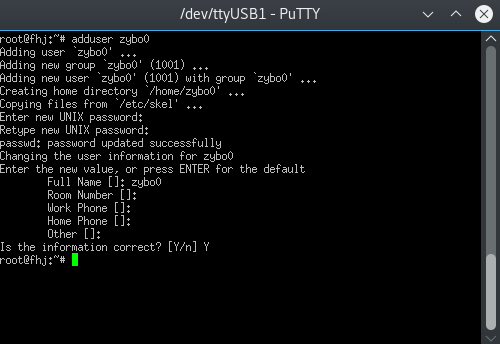
\includegraphics[scale=0.9]{Anexos/Anexo2/Linux/NuevoUsuario.png}
	\caption{Ejemplo de creación del usuario zybo0}
	\label{Ejemplo de creación del usuario zybo0}
\end{figure}


\subsection{Habilitar SSH en placas Zybo}
Para establecer una conexión entre el ordenador central y las placas, tendremos que usar el protocolo SSH, que viene deshabilitado por defecto en Xillinux.

Para habilitarlo tendremos que acceder al archivo \texttt{/etc/ssh/sshd\_config} como super-usuario. Para ello, utilizaremos el siguiente comando:
\begin{center}
	\texttt{nano /etc/ssh/sshd\_config}
\end{center}
A continuación, nos dirigimos a la línea que tiene la siguiente sentencia:
\begin{center}
	\texttt{\#PasswordAuthentification yes}
\end{center}
Borramos la almohadilla (\#), guardamos y cerramos el fichero.
\begin{figure}[h]
	\centering
	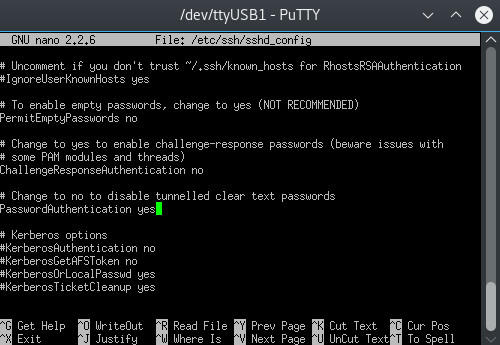
\includegraphics[scale=0.8]{Anexos/Anexo2/Linux/SSH.png}
	\caption{Fichero \texttt{sshd\_config} modificado}
	\label{Fichero ssh_d modificado}
\end{figure}

\newpage
Para establecer los cambios realizados, debemos reiniciar el servicio SSH. Para ello utilizamos:
\begin{center}
	\texttt{/etc/init.d/ssh restart}
\end{center}
\begin{figure}[h]
	\centering
	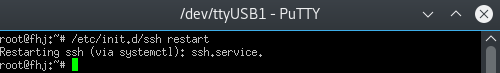
\includegraphics[scale=0.8]{Anexos/Anexo2/Linux/SSHRestart.png}
	\caption{Reiniciando el servicio SSH}
	\label{Reiniciando el servicio SSH}
\end{figure}

A partir de aquí ya podemos establecer conexiones SSH desde el ordenador central al resto de placas Zybo y enviar cualquier tipo de ficheros bien sea desde el ordenador central a las placas o bien, entre placas.